
\section{Rayleigh-Taylor instability}
\label{sec:rayleigh}

\begin{frame}
    \frametitle{Rayleigh-Taylor simulation}

    Boundary interface specifies \texttt{preUpdateBoundaryHandling} and \texttt{postUpdateBoundaryHandling} function

    \vspace{7pt}
    \begin{columns}
        \begin{column}{.5\textwidth}
            \centering{\textbf{preUpdateBoundaryHandling}}
            \begin{itemize}
                \item Executed before any forces are calculated
                \item[] \!\!\!\!\!\!\!\!\! \textcolor{orange}{$\Rightarrow$} Add all required halo particles
                \item Map from \texttt{CellIndex} to manipulations of the cell index and particle position $\rightarrow$ particle position + shift = halo particle position
                \item If multiple periodic boundaries affect a cell, only one will perform all shifts
            \end{itemize}
        \end{column}

        \begin{column}{.5\textwidth}
            \centering{\textbf{postUpdateBoundaryHandling}}
            \begin{itemize}
                \item Called after all updates to the particles
                \item All inserted halo particles will be removed
                \item Only after all bounds have been applied the particle is within the domain (known end)
                \item[] \!\!\!\!\!\!\!\!\! \textcolor{orange}{$\Rightarrow$} Only then do update
            \end{itemize}
        \end{column}
    \end{columns}
    \vspace{7pt}

    \begin{itemize}
        \item New force calculation including gravitational force
        \item Simulation class \texttt{MixedLJSimulation} for multiple particle types:
        \begin{itemize}
            \item Uses Lorentz-Berthelot mixing rule for parameters during setup
            \item Includes thermostat for temperature update and initialization
        \end{itemize}
    \end{itemize}
\end{frame}

\begin{frame}
    \frametitle{Simulation observations}
    \begin{itemize}
        \item Noticeable Bouncing/Splashing when layers collide
        \item Top liquid forms drops initially while mixing
    \end{itemize}
    \begin{figure}
        \label{fig:bounce}
        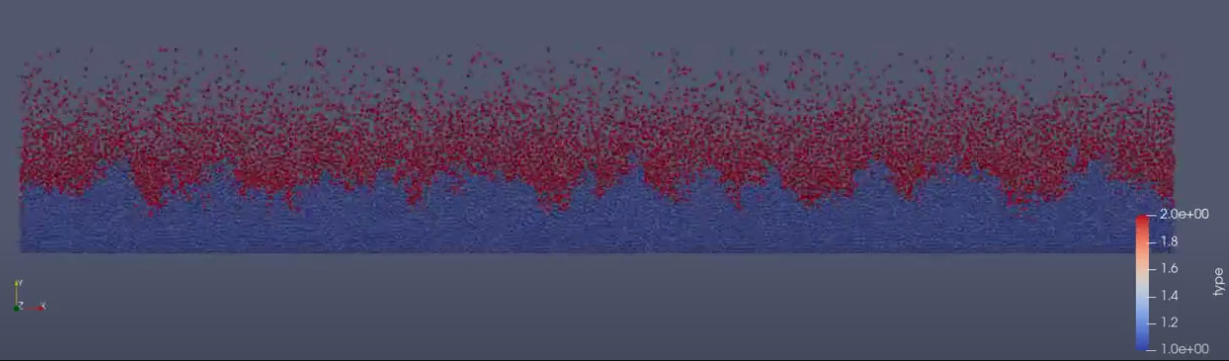
\includegraphics[width=0.9\textwidth]{../../res/rayleigh_bounce}
    \end{figure}
\end{frame}